\documentclass[letterpaper,12pt,fleqn]{article}
\usepackage{matharticle}
\pagestyle{empty}
\newcommand{\vx}{\vec{x}}
\newcommand{\vy}{\vec{y}}
\newcommand{\norm}[1]{\left\|#1\right\|}
\newcommand{\e}{\epsilon}
\newcommand{\comp}[1]{\overline{#1}}
\begin{document}
\section*{Open and Closed Sets}

\begin{definition}[Ball]
  Let $E$ be a normed space, $\vx\in E$, and $r>0$:
  \begin{enumerate}
  \item $B(\vx,r)=\{\vy\in E\mid\norm{\vx-\vy}<r$ is called an
    \emph{open ball}.
  \item $\comp{B}(\vx,r)=\{\vy\in E\mid\norm{\vx-\vy}\le r$ is called a
    \emph{closed ball}.
  \item $S(\vx,r)=\{\vy\in E\mid\norm{\vx-\vy}=r$ is called a
    \emph{sphere}.
  \end{enumerate}
  In all cases, $\vx$ is called the \emph{center} and $r$ is called the
  \emph{radius}.
\end{definition}

\begin{example}
  Let $E=R^2$ and let $B_k(0,1)$ be the unit ball for $\norm{\cdot}_k$ for
  $1\le k\le\infty$:

  \begin{minipage}{2in}
    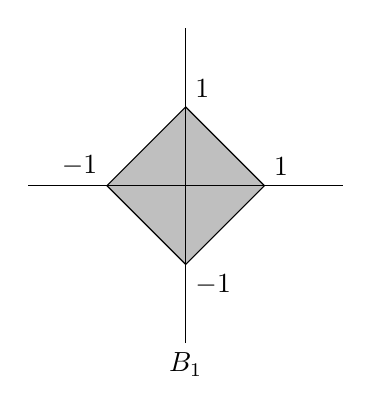
\begin{tikzpicture}
      \draw [fill=lightgray] (1,0) -- (0,-1) -- (-1,0) -- (0,1) -- cycle;
      \draw (-2,0) -- (2,0);
      \draw (0,-2) -- (0,2);
      \node [above right] at (1,0) {$1$};
      \node [above right] at (0,1) {$1$};
      \node [above left] at (-1,0) {$-1$};
      \node [below right] at (0,-1) {$-1$};
      \node [below] at (0,-2) {$B_1$};
    \end{tikzpicture}
  \end{minipage}
  \begin{minipage}{2in}
    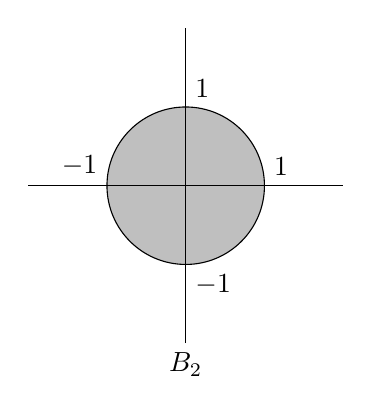
\begin{tikzpicture}
      \draw [fill=lightgray] (0,0) circle [radius=1];
      \draw (-2,0) -- (2,0);
      \draw (0,-2) -- (0,2);
      \node [above right] at (1,0) {$1$};
      \node [above right] at (0,1) {$1$};
      \node [above left] at (-1,0) {$-1$};
      \node [below right] at (0,-1) {$-1$};
      \node [below] at (0,-2) {$B_2$};
    \end{tikzpicture}
  \end{minipage}
  \begin{minipage}{2in}
    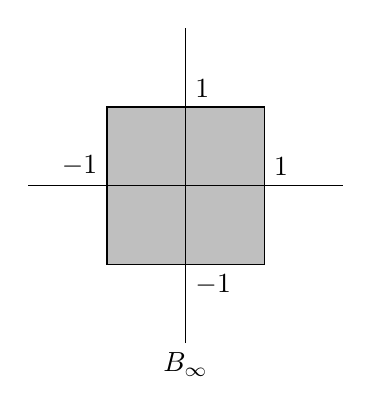
\begin{tikzpicture}
      \draw [fill=lightgray] (-1,-1) rectangle (1,1);
      \draw (-2,0) -- (2,0);
      \draw (0,-2) -- (0,2);
      \node [above right] at (1,0) {$1$};
      \node [above right] at (0,1) {$1$};
      \node [above left] at (-1,0) {$-1$};
      \node [below right] at (0,-1) {$-1$};
      \node [below] at (0,-2) {$B_{\infty}$};
    \end{tikzpicture}
  \end{minipage}
\end{example}

\begin{definition}[Open]
  Let $E$ be a normed vector space and $S\subset E$. To say that $S$ is
  \emph{open} means:
  \[\forall\,\vx\in S,\exists\,\e>0,B(\vx,\e)\subset S\]
  To say that $S$ is \emph{closed} means $E\setminus S$ is open.

  To say that $S$ is \emph{clopen} means it is both open and closed.
\end{definition}

\begin{theorem}
  Let $E$ be a non-trivial normed vector space:
  \begin{enumerate}
  \item The union of any collection of open subsets of $E$ is open.
  \item The empty set and $E$ are clopen.
  \item The intersection of a finite number of open subsets of $E$ is open.
  \item The union of a finite number of closed subsets of $E$ is closed.
  \item The intersection of any collection of closed subsets of $E$ is closed.
  \end{enumerate}
\end{theorem}

\newpage

\begin{theproof}
  \listbreak
  \begin{enumerate}
  \item Assume $\{U_i\mid i\in I\}$ is a collection of open subsets of $E$ and
    let $U=\bigcup_{i\in I}U_i$.

    Assume $\vx\in U$. \\
    $\exists\,i\in I,\vx\in U_i$ \\
    But $U_i$ is open, so $\exists\,\e>0,B(\vx,\e)\subset U_i\subset U$. \\
    Thus $B(\vx,\e)\subset U$.

    Therefore, $U$ is open.

  \item By definition, the empty set is vacuously open, and since
    $E\setminus\emptyset=E$, $E$ is closed by definition. Conversely, since
    $E$ is the union of all possible open subsets of $E$, $E$ must also be
    open. And since $\emptyset=E\setminus E$, $\emptyset$ must also be closed.
    Therefore, $\emptyset$ and $E$ are clopen.

  \item Proof by induction on the number of open sets $n$.

    \begin{description}
    \item Base case: $n=2$

      Assume $U,V\subset E$ are open sets and let $W=U\cap V$. \\
      If $W=\emptyset$ then $W$ is open, so AWLOG that $W\ne\emptyset$. \\
      Assume $\vx\in W$. \\
      $\vx\in U$ and $\vx\in V$. \\
      But $U$ and $V$ are open, so $\exists\,\e_u,\e_v>0$ such that
      $B(\vx,\e_u)\subset U$ and $B(\vx,\e_v)\subset V$. \\
      Let $\e=\min\{\e_u,\e_b\}$. \\
      $B(\vx,\e)\subseteq B(\vx,\e_u)\subset U$ and
      $B(\vx,\e)\subseteq B(\vx,\e_v)\subset V$. \\
      And so $B(\vx,\e)\subset U\cap V=W$.

      Therefore, $W=U\cap V$ is open.

    \item Assume that an intersection of $n$ open subsets of $E$ is open.

    \item Assume ${U_1,\ldots,U_{n+1}}$ are $n+1$ open subsets of $E$.

      Let $U=\bigcap_{k=1}^{n+1}U_k=
      \left(\bigcap_{k=1}^nU_k\right)\cap U_{n+1}$. \\
      But by the inductive assumption, $\bigcap_{k=1}^nU_k$ is an open set.

      Therefore, by the base case, $U$ is an open set.
    \end{description}

  \item Assume $V_1,V_2,\ldots,V_n$ is a finite number of closed subsets of
    $E$.

    Let $V=\bigcup_{k=1}^nV_k$. \\
    By DeMorgan: $\comp{V}=\comp{\bigcup_{k=1}^nV_k}=
    \bigcap_{k=1}^n\comp{V_k}$. \\
    But $V_k$ is closed, so $\comp{V_k}$ is open. \\
    And so $\comp{V}$ is an intersection of a finite number of open subsets of
    $E$ and is thus open.

    Therefore $V=\bigcup_{k=1}^nV_k$ is closed.

  \item Assume $\{V_i\mid i\in I\}$ is a collection of closed subsets of $E$.

    Let $V=\bigcap_{i\in I}^nV_i$. \\
    By DeMorgan: $\comp{V}=\comp{\bigcap_{i\in I}V_i}=
    \bigcup_{i\in I}\comp{V_i}$. \\
    But $V_i$ is closed, so $\comp{V_i}$ is open. \\
    And so $\comp{V}$ is a union of a collection of open subsets of $E$ and is
    thus open.

    Therefore $V=\bigcap_{i\in I}V_i$ is closed.
  \end{enumerate}
\end{theproof}

\begin{examples}
  Let $U_n=(-\frac{1}{n},\frac{1}{n})$. \\
  $\bigcap_{n=1}^{\infty}U_n=\{0\}$, which is closed.

  Therefore, an intersection of an infinite collection of open sets is not
  necessarily open.

  Let $V_n=[-1+\frac{1}{n},1-\frac{1}{n}]$. \\
  $\bigcup_{n=1}^{\infty}V_n=(-1,1)$, which is open.

  Therefore, a union of an infinite collection of closed sets is not
  necessarily closed.
\end{examples}

\begin{theorem}
  Let $E$ be a normed space and let $S\subseteq E$:

  \qquad$S$ is closed $\iff \forall\,(\vx_n)\ \mbox{in}\ S,
  \vx_n\to \vx\implies\vx\in S$

  Thus, $S$ contains all of its limit points.
\end{theorem}

\begin{theproof}
  \listbreak
  \begin{description}
  \item $\implies$ Assume $S$ is closed.

    Assume $(\vx_n)$ is in $S$ and $\vx_n\to\vx$. \\
    ABC: $\vx\notin S$. \\
    Since $S$ is closed, $E\setminus S$ is open. \\
    So, $\exists\,\e>0$ such that $B(\vx,\e)\in E\setminus S$. \\
    And so $\forall\,n\in\N,\norm{\vx_n-\vx}>\e$. \\
    But, by assumption, $\vx_n\to\vx$ and so $\norm{\vx_n-\vx}<\e$ for $n$
    sufficiently large. \\
    CONTRADICTION!

    Therefore, $\vx\in S$.

  \item $\impliedby$ Assume $S$ contains all of its limit points.

    ABC: $S$ is open. \\
    Thus, $E\setminus S$ is closed, and so $\exists\,\vx\in E\setminus S$ such
    that $\forall\,\e>0, B(\vx,\e)\cap S\ne\emptyset$. \\
    Construct a sequence $(\vx_n)\in S$ such that
    $\vx_n\in B(\vx,\frac{1}{n})$. \\
    Clearly, $\vx_n\to\vx\notin S$, so $\vx$ is a limit point for $S$ that is
    not in $S$. \\
    CONTRADICTION!

    Therefore, $S$ is closed.
  \end{description}
\end{theproof}

\end{document}
